\section*{Exercice 189 -- Modélisation}
\setcounter{exo}{0}
%CCS PSI 2008

Pour respecter les exigences du cahier des charges, les vantaux doivent avoir un
mouvement de translation de direction $\vect{y}$ par rapport à la voiture. 

\begin{center}
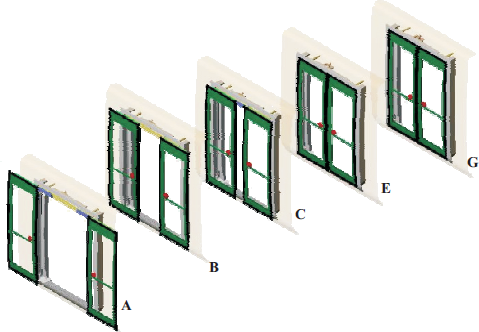
\includegraphics[width=\linewidth]{985_01}%
\end{center}

Ce mouvement est assuré par le guidage de la poutre de fermeture grâce à
deux boîtes à galets placées aux points $H$ et $J$ de la figure suivante qui donne le
modèle retenu pour chacune d’elles. 

\begin{center}
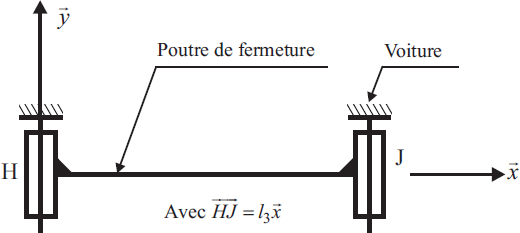
\includegraphics[width=\linewidth]{985_02}%
\end{center}

\begin{obj}
L’objet de cette partie est de trouver la liaison équivalente à l’association de ces
deux liaisons.
\end{obj}

\subparagraph{}
\textit{Déterminer le degré d’hyperstatisme de ce modèle. En déduire les contraintes géométriques à satisfaire lors de la réalisation.}
\ifprof
\begin{corrige}
\end{corrige}
\else
\fi

\subparagraph{}
\textit{Proposer une liaison élémentaire cinématiquement équivalente à ces deux
liaisons et exprimer son torseur cinématique caractéristique.}
\ifprof
\begin{corrige}
\end{corrige}
\else
\fi

\subparagraph{}
\textit{Proposer et justifier un modèle pour la liaison élémentaire au point qui rende la liaison résultante isostatique.}
\ifprof
\begin{corrige}
\end{corrige}
\else
\fi

Le document réponse représente les schémas cinématiques du mécanisme pour les trois étapes de fonctionnement.


\begin{center}
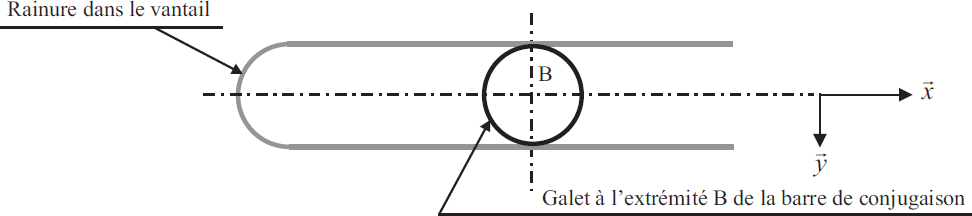
\includegraphics[width=\linewidth]{985_03}%
\end{center}


\subparagraph{}
\textit{Compléter les schémas, en représentant la barre de conjugaison et en indiquant pour
chaque étape la liaison équivalente en entre la barre de conjugaison et le vantail.}
\ifprof
\begin{corrige}
\end{corrige}
\else
\fi

\begin{rem}
\begin{itemize}
\item Pour la phase coulissement, la barre de conjugaison est parallèle à l’axe .
\item Le galet de forme cylindrique est en liaison rotule (ou sphérique) avec la barre de conjugaison
\end{itemize}
\end{rem}


\begin{center}
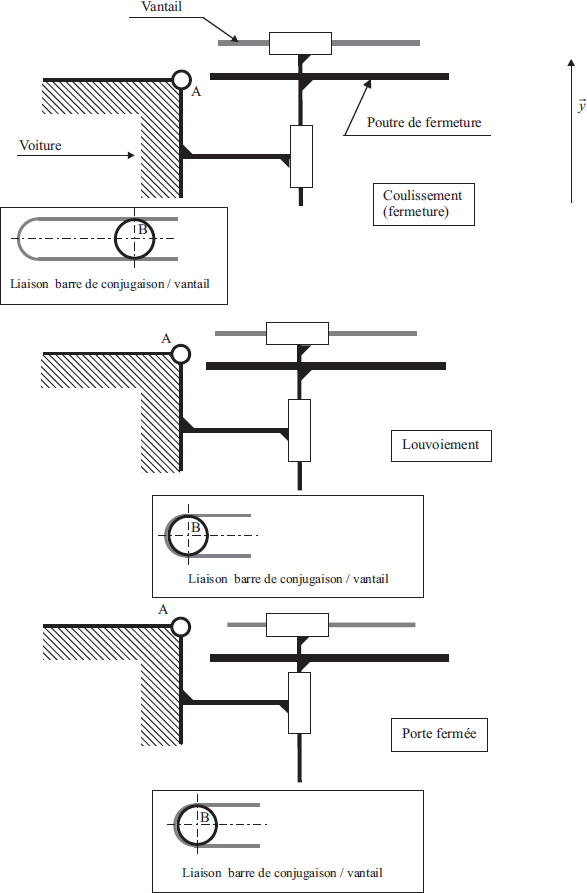
\includegraphics[width=\linewidth]{985_04}%
\end{center}



\begin{enumerate}
\item $h=3$, parallélisme des axes et entraxe.
\item Glissière de direction $\vect{y}$.
\item Liaison sphère plan de normale $\axe{J}{z}$.
\item ...
\end{enumerate}
